\documentclass{oci}
\usepackage[utf8]{inputenc}
\usepackage{lipsum}
\usepackage{tikz}

\title{Secuencia de ADN}

\begin{document}
\begin{problemDescription}
  El ácido desoxirribonucleico, o ADN, fue descubierto por Friedrich Miescher,
  quien en 1869 fue el primero en lograr aislarlo.
  Durante las siguientes décadas, el ADN permaneció sin ser muy estudiado, hasta que
  en 1944 algunos experimentos de Oswald Avery, Colin MacLeod y Maclyn McCarty lograron
  demostrar que la manipulación de ADN dentro de una bacteria podía afectar su comportamiento.
  Aproximadamente una década después, James Watson y Francis Crick presentaron
  su famoso modelo del ADN.
  De acuerdo a su modelo, una cadena de ADN está formada por una secuencia
  de nucleótidos, existiendo 4 tipos: adenina, guanina, citosina y timina.

  La secuenciación de ADN es el proceso que permite determinar el orden de los
  nucleótidos en una cadena de ADN.
  Gracias a importantes avances científicos que comenzaron en la década de los 70, hoy
  es posible secuenciar el ADN de organismos completos.

  Una vez que la secuenciación de una cadena está completa, es posible 
  guardarla como un arreglo de números entre 0 y 3, donde cada número
  representa un nucleótido (adenina (0), guanina (1), citosina (2) y timina (3)).
  Con esta representación es posible hacer diferentes análisis sobre la cadena que
  permiten, entre otras cosas, encontrar defectos que pueden ser asociados a la
  presencia de ciertas enfermedades.

  Recientes técnicas en el análisis de ADN requieren poder encontrar patrones
  cortos de largo tres dentro de una cadena de ADN.
  Esto permite encontrar puntos de interés para su posterior análisis.
  Considera, por ejemplo, el siguiente arreglo que representa una cadena de ADN:

  \begin{center}
    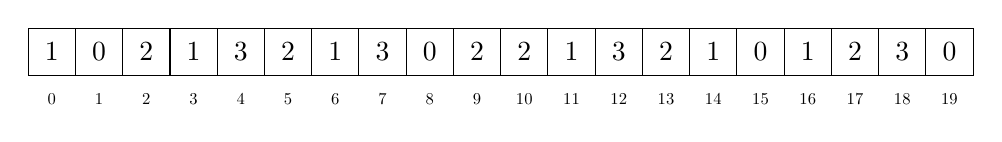
\begin{tikzpicture}[scale = 0.6]
      \foreach \i in {0,...,19}{
        \draw (\i,0) rectangle +(1,1);
        \node at (\i+0.5,-0.5) {\scalebox{0.6}{$\i$}};
      }
      \node at (0+0.5,0.5) {$1$};
      \node at (1+0.5,0.5) {$0$};
      \node at (2+0.5,0.5) {$2$};
      \node at (3+0.5,0.5) {$1$};
      \node at (4+0.5,0.5) {$3$};
      \node at (5+0.5,0.5) {$2$};
      \node at (6+0.5,0.5) {$1$};
      \node at (7+0.5,0.5) {$3$};
      \node at (8+0.5,0.5) {$0$};
      \node at (9+0.5,0.5) {$2$};
      \node at (10+0.5,0.5) {$2$};
      \node at (11+0.5,0.5) {$1$};
      \node at (12+0.5,0.5) {$3$};
      \node at (13+0.5,0.5) {$2$};
      \node at (14+0.5,0.5) {$1$};
      \node at (15+0.5,0.5) {$0$};
      \node at (16+0.5,0.5) {$1$};
      \node at (17+0.5,0.5) {$2$};
      \node at (18+0.5,0.5) {$3$};
      \node at (19+0.5,0.5) {$0$};
    \end{tikzpicture}
  \end{center}

  En esta cadena se quiere encontrar las ocurrencias del patrón $1\,3\,2$.
  Este patrón ocurre dos veces en la cadena, primero en la posición 3 y luego
  en la 11.
  
  Dado un patrón, tu tarea es contar la cantidad de veces que dicho patrón ocurre
  dentro de una cadena de ADN.
  ?`Podrías ayudar a los científicos a encontrar estos patrones?
\end{problemDescription}

\begin{inputDescription}
  La primera línea de la entrada contiene un entero $N$ ($0 < N \leq 100\,000$)
  correspondiente al largo de la cadena de ADN.
  La segunda línea contiene $N$ enteros, todos entre 0 y 3, que describen la
  secuencia de ADN.
  Finalmente, la tercera línea contiene tres enteros entre 0 y 3, que describen
  el patrón que se desea encontrar.
\end{inputDescription}

\begin{outputDescription}
  La salida debe contener un único entero correspondiente a la cantidad de veces
  que el patrón ocurre dentro de la cadena de ADN.
\end{outputDescription}

\begin{scoreDescription}
  Este problema no contiene subtareas.
  Se dará puntaje proporcional a la cantidad de casos de prueba correctos, siendo
  100 el puntaje máximo.
\end{scoreDescription}

\begin{sampleDescription}
\sampleIO[0.5][0.4]{sample-1}
\sampleIO[0.5][0.4]{sample-2}
\end{sampleDescription}

\end{document}
